\documentclass[Main]{subfiles}
\begin{document}


\chapter{Decoder}

\section{Operation of the Meggitt decoder}

When decoding cyclic codes, the straight forward approach involves creating a table, that matches all possible error patterns to the corresponding syndrome vector. This approach is impractical when creating a decoding circuit, because the complexity of the circuit tends to grow exponentially with code length and number of errors corrected \cite{lec7}.

This problem can be remedied using the Meggitt decoder. The basis of the Meggitt decoder is Theorem 3.1 presented during lecture 7\cite{lec7}.

\noindent
\framebox{\parbox{\dimexpr\linewidth-2\fboxsep-2\fboxrule}{
 \textbf{Theorem 3.1:} If the received polynomial
$r (x) = r_0 + r_1X + r_2X^2 ... + r_{n-1} X^{n-1}$  generates the syndrome
polynomial $S(X)$. Then a cyclic right shift of the received polynomial $r^{(1)}(X)$ generates the syndrome polynomial $S^{(1)}(X)$. $S^{(1)}(X)$ is actually the remainder of dividing $XS(X)$ by generator polynomial $g(X)$.
}}

Theorem 3.1 can be summarized as such:

$ r(X) \hspace*{2em}  \Rightarrow^{rightshift} \hspace*{2em} r^{(1)}(X)$ \\
$ \Downarrow \hspace*{12em} \Downarrow$ \\
$ S(X) \hspace*{9em} S^{(1)}(X)$ \\

The syndrome vector can be calculated using equation \ref{eq:syndromeEq}.

\begin{equation} \label{eq:syndromeEq}
r(X) = q(X)g(X)+s(X)
\end{equation}

The syndrome calculation in the Meggitt decoder is implemented by the circuit in figure \ref{fig:syndromeCirc}. The received vector $r(X)$ is shifted in one bit at a time. When $r(X)$ has been shifted in, the syndrome register.

\begin{figure}[h!]
    \centering
    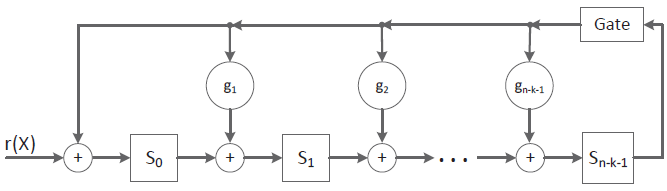
\includegraphics[width=0.8\textwidth]{figures/syndromeCircuit.png}
    \caption{Syndrome calculating circuit}
    \label{fig:syndromeCirc}
\end{figure}

\code{hest}



\section{Decoder overview}

\begin{figure}[h]
    \centering
    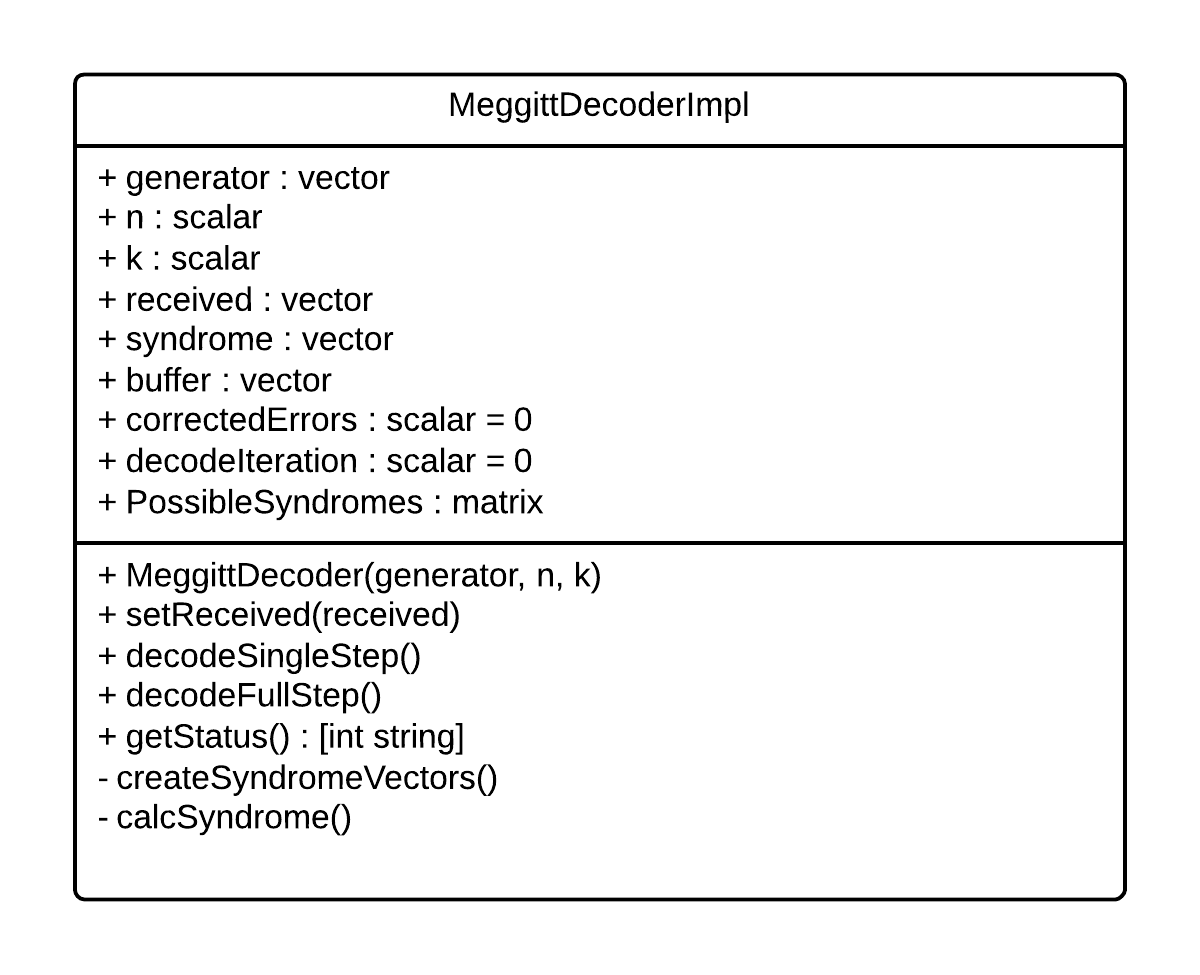
\includegraphics[width=0.8\textwidth]{figures/MeggitDecoderUML.png}
    \caption{Meggitt decoder UML class diagram}
    \label{fig:meggittUML}
\end{figure}



\fxnote{FIXME: Husk key difficulties her}


\end{document} 